\chapter{Justificación}

\section{Ambiental}
Ambientalmente este proyecto está enfocado a reducir el consumo de energía eléctrica, 
dado que la  alimentación requerida consiste en  energía solar, la cual no tiene un 
impacto sobre el medio ambiente, puesto que en Colombia las principales generadoras 
de energía son de tipo hidráulica (aprovecha la energía potencial del agua) y calorífica 
(además de la combustión de carbón también requiere volúmenes de agua). 

Por otro lado se ve involucrado el hecho que entre menos tiempo un automóvil permanezca 
detenido y encendido su motor, disminuiría la emisión de CO2.
\section{Económico}
Económicamente este proyecto tiende a automatizar algunos aspectos en el proceso de 
semaforizar un cruce o una serie de cruces, así que el personal empleado para tal 
tarea disminuirá, uno de los aspectos por los que este fenómeno ocurrirá es que la programación, 
monitoreo y control preventivo de los semáforos se realizara de forma remota.\\

Teniendo en cuenta que el sistema tiene como alimentación paneles fotovoltaicos, 
el consumo de la red nacional de energía es nulo, por lo tanto no existe tal costo.
\section{Académico}
Académicamente el sistema genera toda una investigación, los sistemas de trasporte inteligente 
en Colombia no es un tema del diario vivir, por lo tanto el proyecto intenta cambiar algunos estándares 
y adaptarlos a las condiciones colombianas, uno de estos retos es el manejo en los protocolos (NTCIP, SCOOTS, SCATS, OCIT, ETC…) 
de comunicación enfocados al transporte.

\section{Social}
Se habla por aspecto social el reducir los tiempos de espera en un cruce y mejorar la movilidad, 
que es un aspecto que hoy por hoy es nuestro dolor de cabeza, en Bogotá por colocar un ejemplo 
los accidentes viales son a diario, un estudio de la universidad distrital hace referencia a los 
accidentes por localidad \cite{4}, en el cual se evidencia que los puntos focales de accidentes 
están asociados a congestiones de automóviles, dando como principales causas, las condiciones de la vía, 
imprudencia de la gente y por último y en lo que se enfoca este documento mal funcionamiento de los semáforos\cite{5}

\begin{figure}[h]
    \centering
    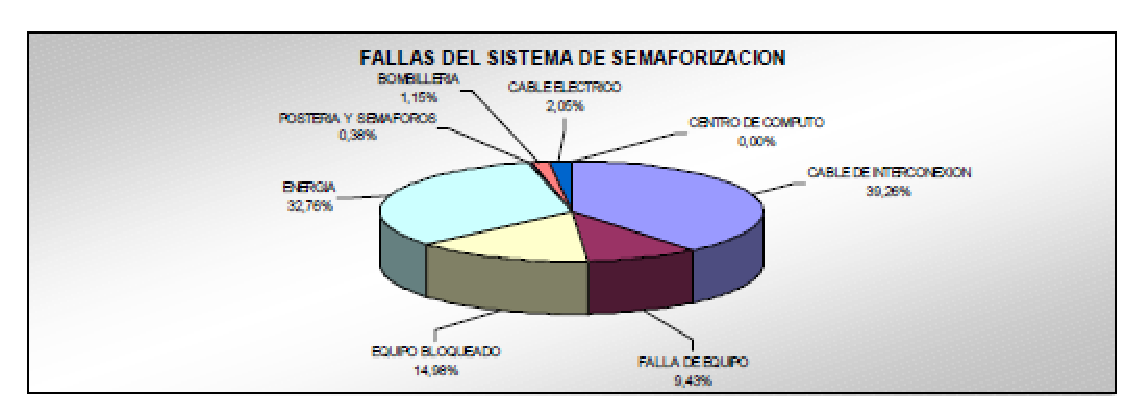
\includegraphics[width=1\textwidth]{ima/estadistica_php9hcqYv}
    \caption{Estadística promedio  de fallas del sistema de semaforización de Bogotá D.C. \cite{5}}
    \label{fig:mesh2}
\end{figure}

\section{Personal}
A nivel personal es un reto cumplir con las especificaciones solicitadas por la compañía, al igual cumplir con este 
proyecto significa mejorar la movilidad en los puntos en los cuales está enfocado el grupo JAMPIG.